\chapter{PENDAHULUAN}

\section{Langkah pertama}
\begin{enumerate}
    \item membuka aplikasi apex oracle
    \item membuat akun baru
    \item klik Request a workspace
\begin{figure}[!htbp]
    \centering
    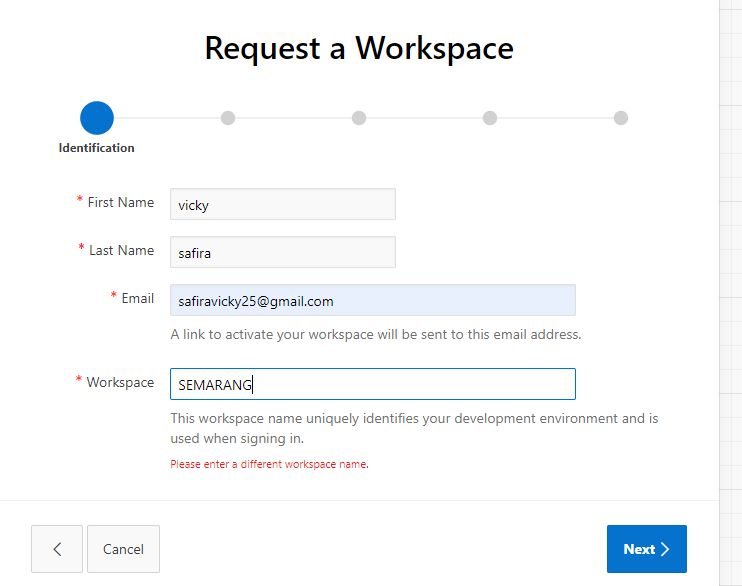
\includegraphics[scale=0.5]{figure/21.PNG}
    \caption{\textit{Request a workspace}}
    \label{gambar 1}
\end{figure}
    \item Lalu klik pilihan seperti dibawah ini, lalu next 
\begin{figure}[!htbp]
    \centering
    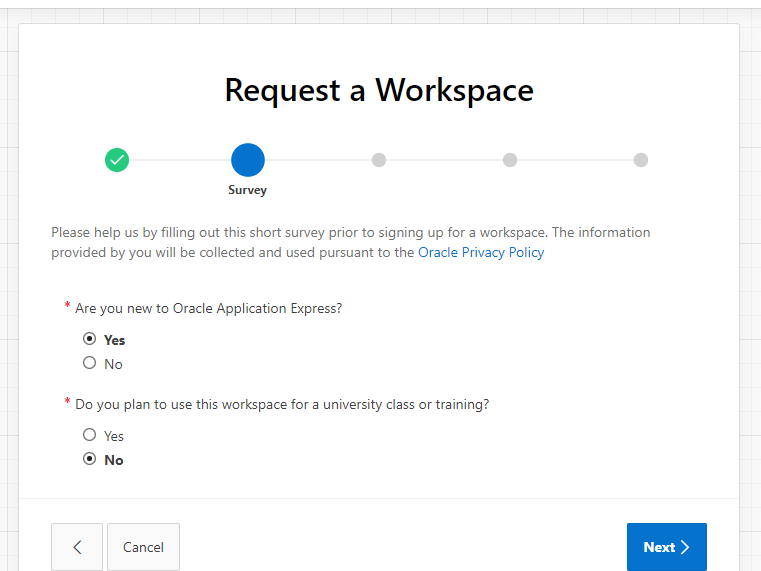
\includegraphics[scale=0.5]{figure/2.PNG}
    \label{gambar 2}
    \caption{\textit{Request a workspace}}
\end{figure} \vspace{6cm}
\item Lalu klik pilihan seperti dibawah ini, lalu next
\begin{figure}[!htbp]
    \centering
    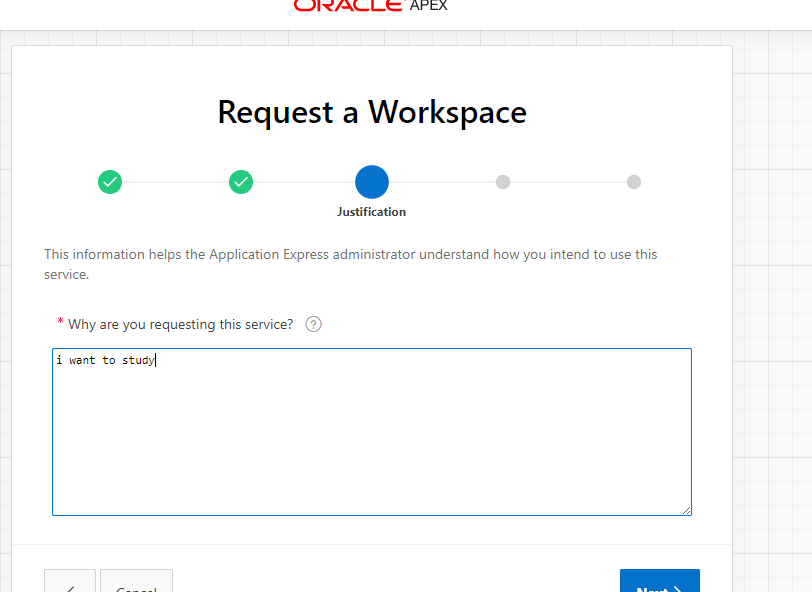
\includegraphics[scale=0.5]{figure/3.PNG}
    \label{gambar 3}
    \caption{\textit{Request a workspace}}
    \vspace{3cm}
\end{figure}
\item Lalu centang tulisan I accept the terms seperti dibawah lalu next
\begin{figure}[!htbp]
    \centering
    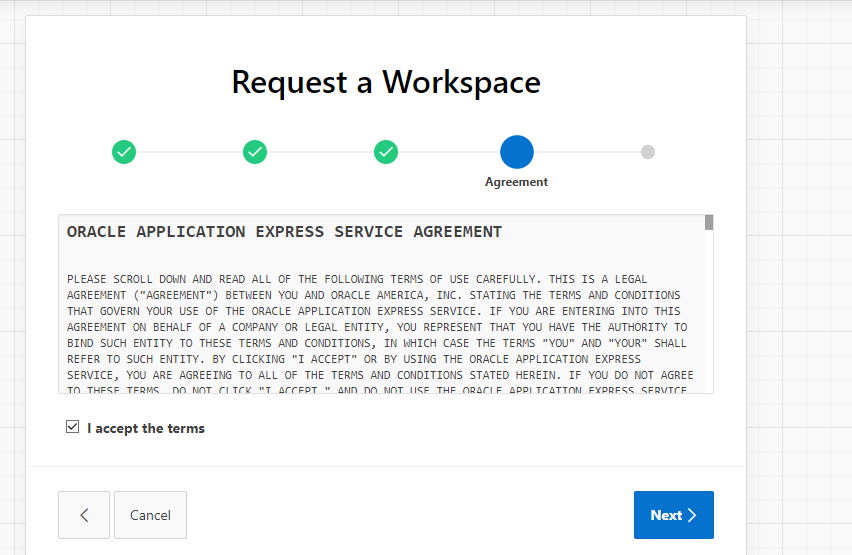
\includegraphics[scale=0.5]{figure/5.PNG}
    \label{gambar 4}
    \caption{\textit{Request a workspace}}
\end{figure}
\item Jika sudah seperti ini lalu klik Submit Request
\begin{figure}[!htbp]
    \centering
    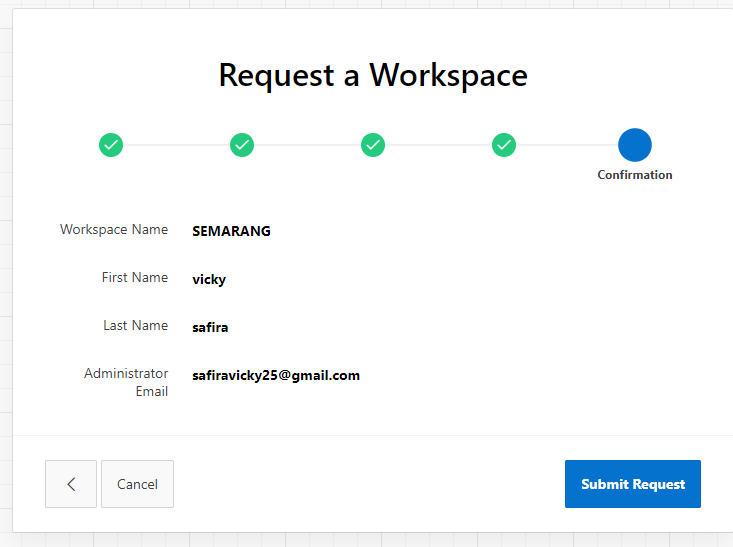
\includegraphics[scale=0.5]{figure/22.PNG}
    \label{gambar 5}
    \caption{\textit{Request a workspace}}
\end{figure} \vspace{6cm}
\item Jika sudah selesai  klik Continue to Sign In Screen
\begin{figure}[!htbp]
    \centering
    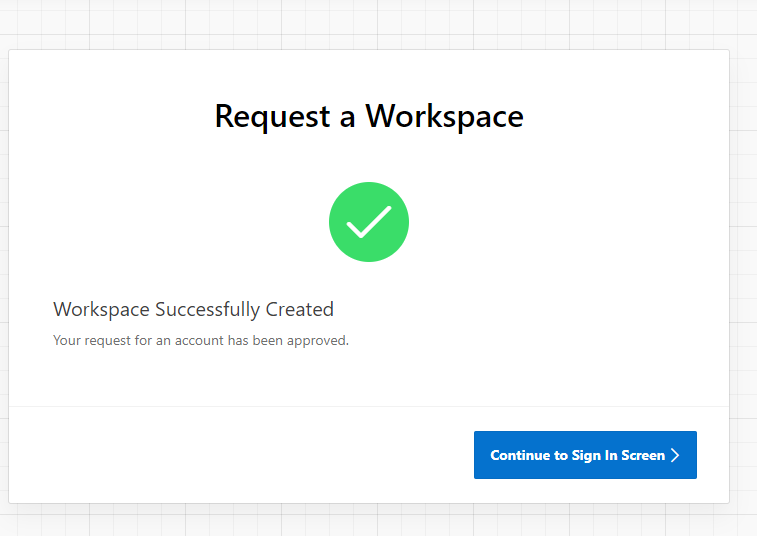
\includegraphics[scale=0.5]{figure/8.PNG}
    \label{gambar 6}
    \caption{\textit{Request a workspace}}
\end{figure}
\item Lalu akan muncul tampilan seperti ini, setelah itu klik Submit Request
\begin{figure}[!htbp]
    \centering
    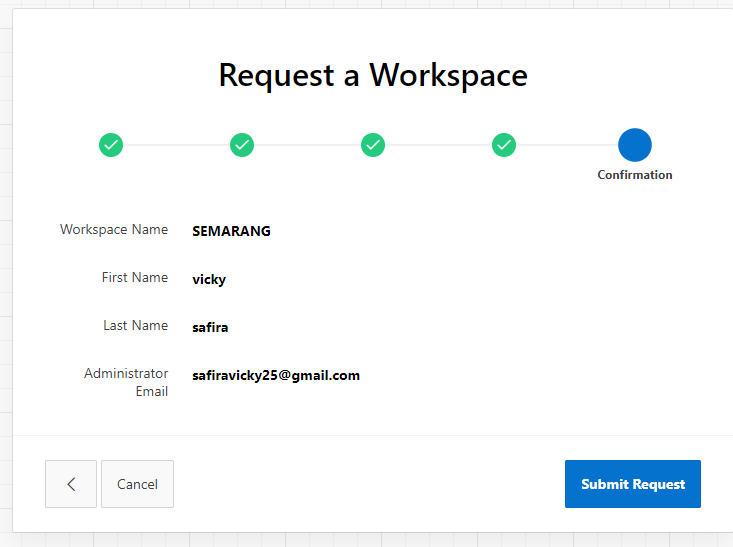
\includegraphics[scale=0.5]{figure/22.PNG}
    \label{gambar 7}
     \caption{\textit{Request a workspace}}
\end{figure} \vspace{6cm}
\item Setelah itu akan muncul tampilan seperti ini, lalu klik Apply Changes
\begin{figure}[!htbp]
    \centering
    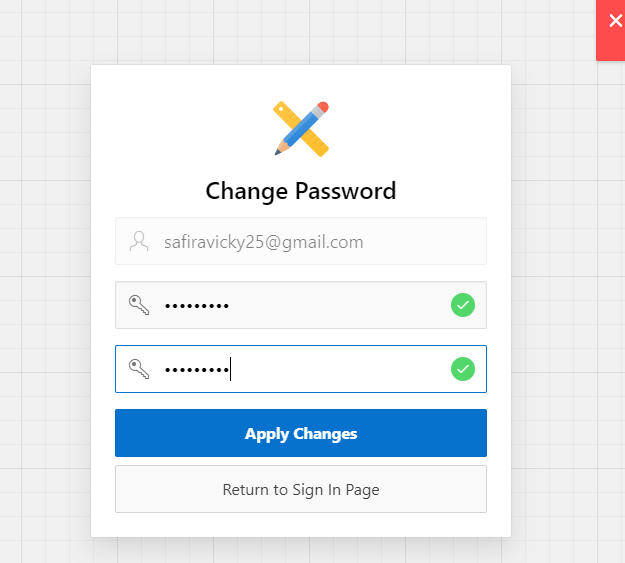
\includegraphics[scale=0.5]{figure/9.PNG}
    \label{gambar 7}
     \caption{\textit{Request a workspace}}
\end{figure}
\item Setelah itu klik App Builder
\begin{figure}[!htbp]
    \centering
    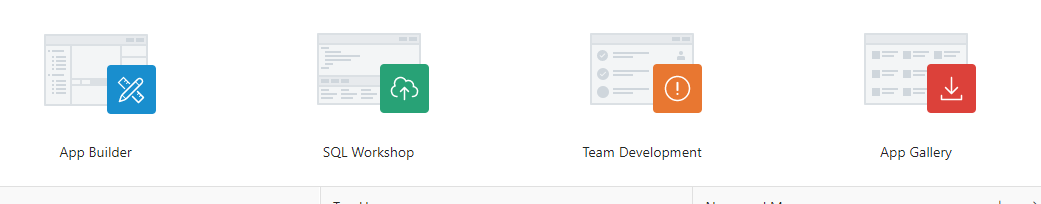
\includegraphics[scale=0.5]{figure/10.PNG}
    \label{gambar 7}
     \caption{\textit{Request a workspace}}
\end{figure}
\item Setelah itu klik Create
\begin{figure}[!htbp]
    \centering
    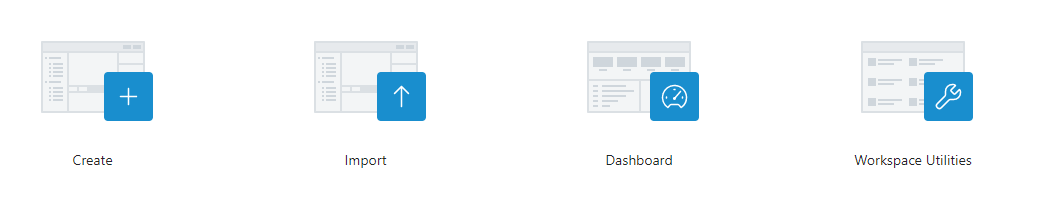
\includegraphics[scale=0.5]{figure/11.PNG}
    \label{gambar 7}
     \caption{\textit{Request a workspace}}
\end{figure}
\item Setelah itu klik From a File
\begin{figure}[!htbp]
    \centering
    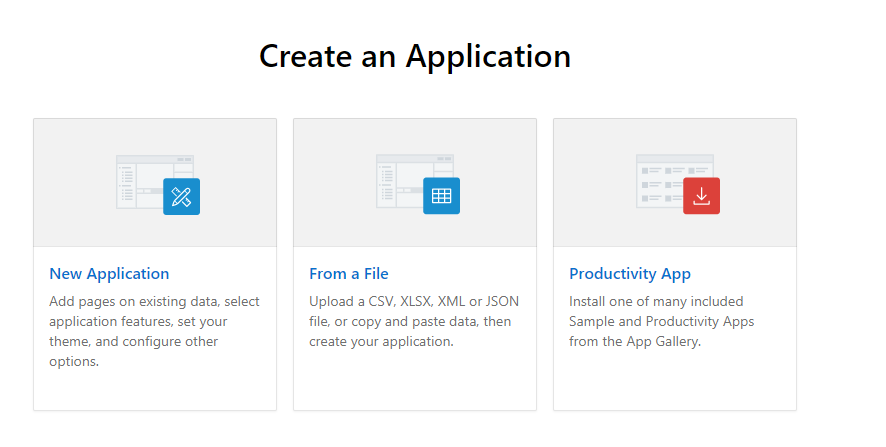
\includegraphics[scale=0.5]{figure/12.PNG}
    \label{gambar 7}
     \caption{\textit{Request a workspace}}
\end{figure} \vspace{6cm}
\item Setelah itu klik Choose File
\begin{figure}[!htbp]
    \centering
    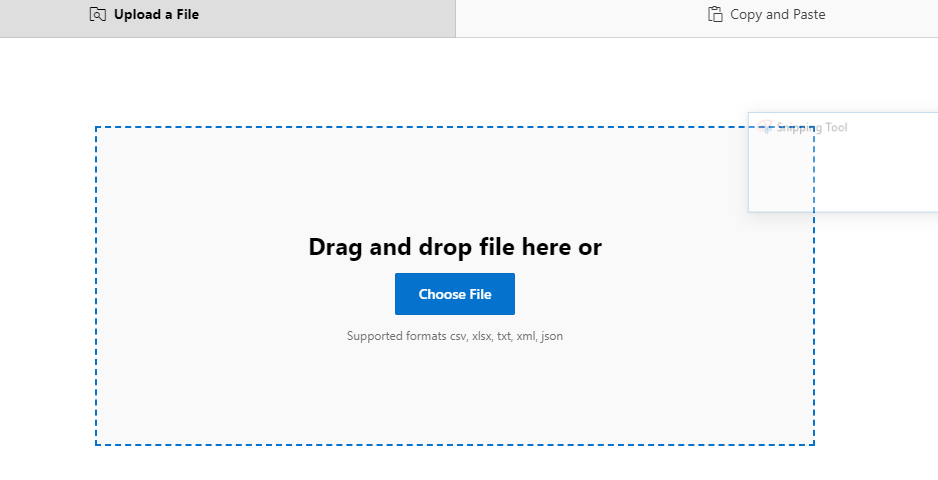
\includegraphics[scale=0.5]{figure/13.PNG}
    \label{gambar 7}
     \caption{\textit{Request a workspace}}
\end{figure}
\item Setelah itu akan muncul tampilan seperti ini, lalu klik Load Data
\begin{figure}[!htbp]
    \centering
    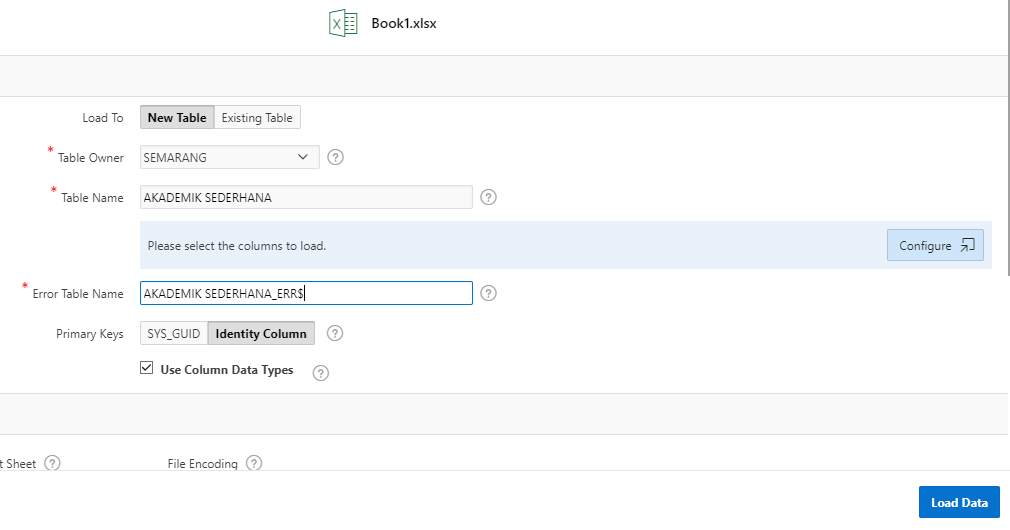
\includegraphics[scale=0.5]{figure/24.PNG}
    \label{gambar 7}
     \caption{\textit{Request a workspace}}
\end{figure} \vspace{6cm}
\item Setelah itu akan muncul tampilan seperti ini, lalu klik Create Application
\begin{figure}[!htbp]
    \centering
    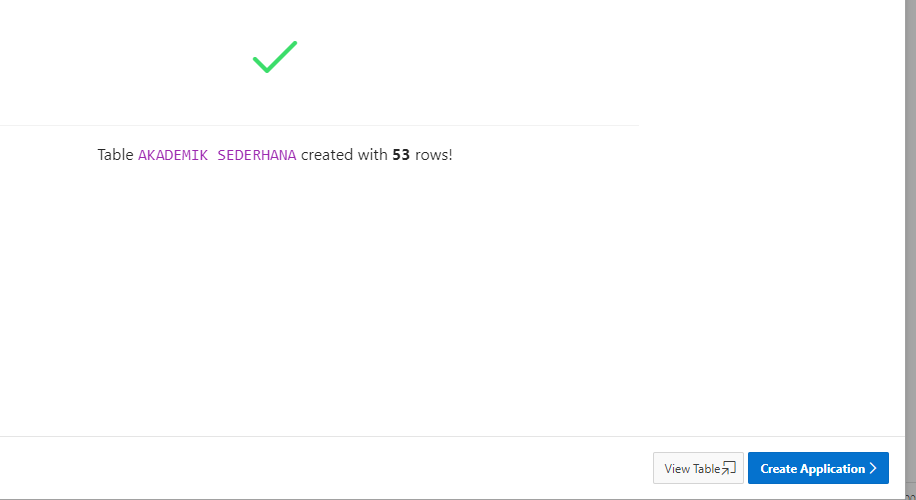
\includegraphics[scale=0.5]{figure/25.PNG}
    \label{gambar 7}
     \caption{\textit{Request a workspace}}
\end{figure} \vspace{6cm}
\item Lalu klik Create dipojok kanan bawah
\begin{figure}[!htbp]
    \centering
    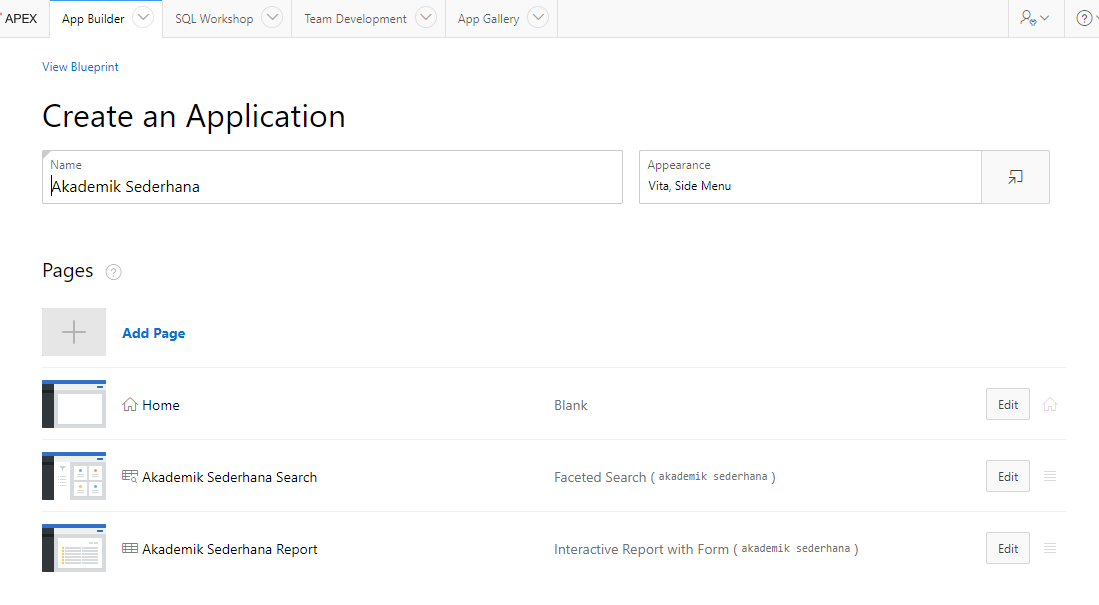
\includegraphics[scale=0.5]{figure/26.PNG}
    \label{gambar 7}
     \caption{\textit{Request a workspace}}
\end{figure}
\item Setelah itu klik Run Application
\begin{figure}[!htbp]
    \centering
    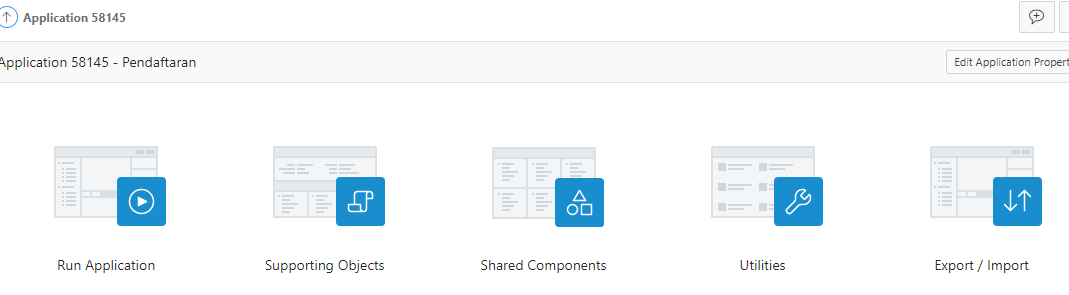
\includegraphics[scale=0.5]{figure/17.PNG}
    \label{gambar 7}
     \caption{\textit{}}
\end{figure} \vspace{6cm}
\item Lalu masukkan username dan password lalku klik sign in
\begin{figure}[!htbp]
    \centering
    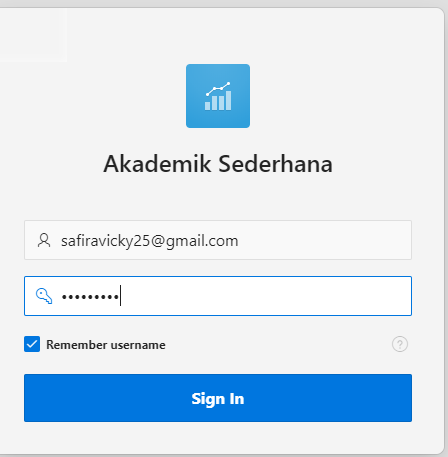
\includegraphics[scale=0.5]{figure/27.PNG}
    \label{gambar 7}
     \caption{\textit{}}
\end{figure}
\item Setelah muncul tampilan seperti ini tandanya sudah selesai
\begin{figure}[!htbp]
    \centering
    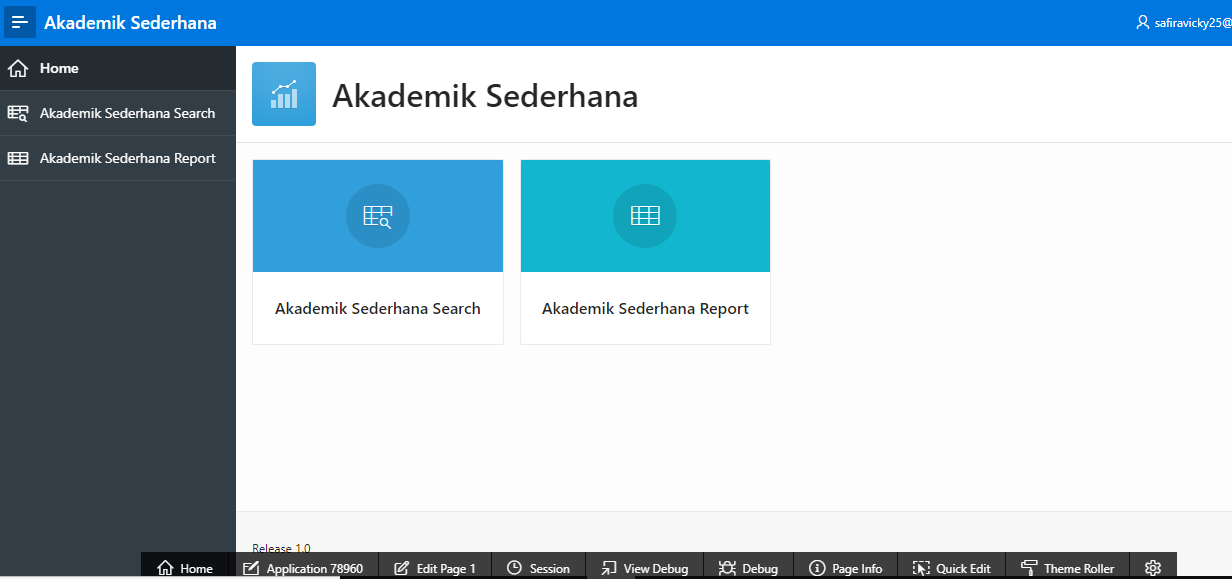
\includegraphics[scale=0.5]{figure/28.PNG}
    \label{gambar 7}
     \caption{\textit{}}
\end{figure}
\end{enumerate}
\section{Langkah kedua}
setelah selesai di langkah pertama,dan apliasinya selesai selanjutnya membuka aplikasi yang telah selesai kau buat dengan nama akademik.
\begin{enumerate}
    \item masuk ke akademik dan masukan email dan password
    \item terus pilih data Search
didalam data search terdapat data nilai mahasiswa 
    \title{[Berikut Adalah link, usernamse dan password saya]} 
    \title{https://apex.oracle.com/pls/apex/f?p=78960:LOGIN_DESKTOP:722740888836575:::::}
    \item username : safiravicky25@gmail.com pwd : vicky2016
\end{enumerate}

